\PassOptionsToPackage{dvipsnames}{xcolor}
\documentclass[10pt]{article}
%\documentclass[10pt,draft]{article}
\usepackage[utf8]{inputenc} % utf8 support

% === Document Layout ===
\usepackage[hmargin=0.75in,vmargin=0.75in]{geometry}
\usepackage{indentfirst}
\usepackage{lipsum}
\usepackage{url}
\usepackage[
    colorlinks,
    linkcolor=red!50!black,
    citecolor=blue!50!black,
    urlcolor=blue!50!black
]{hyperref}
\usepackage{amsmath}
\usepackage{pdfpages}
\usepackage{physics}
\usepackage{graphicx}
\usepackage{xcolor}
\usepackage{mathtools} % for the coloneq command
\usepackage{xparse}
\usepackage{ifthen} % For checking optional parameters
\usepackage{enumerate}
\usepackage{amsthm} % The AMS theorems package
\usepackage{amsthm}
\usepackage{caption}
\captionsetup{width=0.8\textwidth}
\usepackage{subcaption}
\usepackage{float}
\usepackage{tabularx}
\usepackage{authblk} % For affiliations
\usepackage{amsfonts}
\usepackage{indentfirst}
\usepackage{amssymb} % for ordering symbols
\usepackage{colonequals} % for the \ratio command

% amsthm
\newtheorem{theorem}{Theorem}[section]
\newtheorem{lemma}[theorem]{Lemma}
\newtheorem{proposition}[theorem]{Proposition}
\newtheorem{corollary}[theorem]{Corollary}
\newtheorem{conjecture}[theorem]{Conjecture}
\theoremstyle{definition}
\newtheorem{definition}{Definition}[section]
\theoremstyle{remark}
\newtheorem{remark}{Remark}

% === Bibliography ===
\usepackage[
    backend=biber,
    style=authoryear,
    citestyle=authoryear,
]{biblatex}
\addbibresource{references.bib}

\newcommand{\speccite}[1]{\citetitle{#1} \parencite{#1}}

\newcommand{\dt}[1]{\frac{\mathrm d #1}{\mathrm d t}}
\usepackage{pgfplots}
\usepackage{tikz}
\usepackage{tikz-3dplot}
\usetikzlibrary{calc}
\tikzset{every picture/.style={baseline={(current bounding box.center)}}}

\author[1,2]{Thomas C. Fraser}
\affil[1]{Perimeter Institute for Theoretical Physics, Waterloo, Ontario, Canada, N2L 2Y5}
\affil[2]{Dept. of Physics and Astronomy, University of Waterloo, Waterloo, Ontario, Canada, N2L 3G1}
\date{\today}

\title{On the Causality of Dynamical Systems}

\begin{document}
\maketitle

\section*{Disclaimers}

\section{A Chaotic Origin Story}

\subsection{Lorenz's Discovery}
In \speccite{lorenz1963deterministic}, \citeauthor{lorenz1963deterministic} (this is Edward Norton Lorenz, not to be confused with the physicist Ludvig Lorenz, or the actor Edward Norton) presented a simplified dynamical model for atmospheric convection, which today is known as the Lorenz system:
\begin{align}
    \begin{split}
        \dt{X} &= \sigma ( Y - X ), \\
        \dt{Y} &= X ( \rho - Z ) - Y, \\
        \dt{Z} &= XY - \beta Z.
    \end{split}
\end{align}
The Lorenz system was remarkable because despite its determinism and simplicity, it exhibits flows which are non-periodic, chaotic and yet bounded as in Figure~\ref{lorenz_system}. Moreover, Lorenz identifies the non-linearity of the equations as being essential for these features postulates their ubiquity.
\begin{figure}[H]
    \centering
    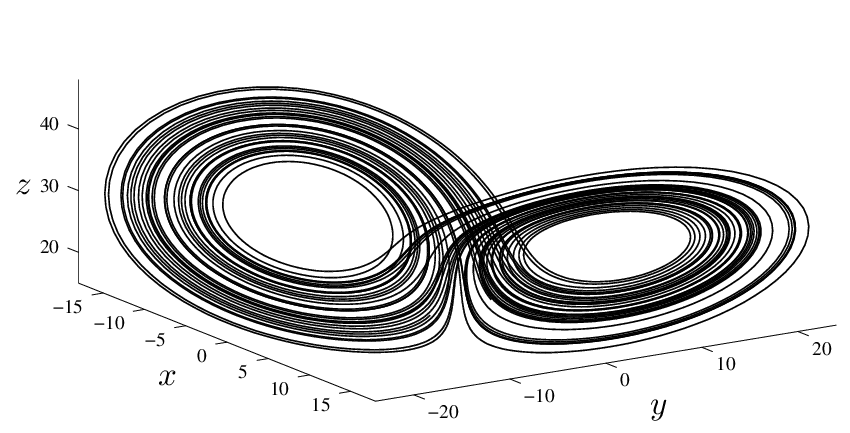
\includegraphics[scale=0.35]{figures/lorenz_system.png}
    \caption{The strange attractor of the Lorenz system for $\sigma = 10, \beta = 8/3, \rho = 28$ with $X(0) = 1.1, Y(0) = -1.9, Z(0) = 13.1$. Figure by \href{https://www.researchgate.net/figure/A-trajectory-of-the-Lorenz-system-in-phase-space-revealing-the-strange-attractor-The_fig1_262074522}{P. T. Clemson}.}
    \label{lorenz_system}
\end{figure}

Later in \speccite{ruelle1971nature}, \citeauthor{ruelle1971nature} develop a variety of mathematics to study such quasi-periodic behaviors and refers to them as \textit{strange attractors}. Importantly, they conjectured that universally, strange attractors where the cause of turbulent behvaiors seen in fluid flow. This conjecture recieved further support after \speccite{gollub1975onset}.

\subsection{What are attractors anyway?}
What exactly is notion of an \textit{attractor}? Intuitively, attractors generalize the more familiar notions of stability for differential equations such as \textit{stable fixed points} and \textit{limit cycles} in the sense that an attractor $A$ is a compact subset such that points starting sufficiently close to $A$ will remain in a given neighborhood of $A$. For a detailed account of the various notions and formulations of an attractor, see \speccite{milnor1985concept}. Nevertheless, the following definition will be adequate. 

A dynamical system on a manifold $M$ (for example $\mathbb R^n$) is specified by a \textbf{flow} (a solution to the system of ODEs)
\begin{equation}
    \Phi_{(\cdot)}(\cdot) : \mathbb R \times M \to M,
\end{equation}
where $\Phi_t$ is a diffeomorphism of $M$ for all $t \in \mathbb R$ such that 
\begin{equation}
    \forall V \in M : \Phi_{0} ( V ) = V, \quad \text{and} \quad \forall s,t \in \mathbb R: \Phi_t \circ \Phi_s = \Phi_{s+t}. 
\end{equation}
An \textbf{attractor} is any $A \subseteq M$ which is
\begin{enumerate}
    \item forward invariant
        \[ \forall a \in A, \forall t \geq 0 : \Phi_{t} ( a ) \in A, \]
    \item admits an neighborhood $B(A)$, called the \textbf{basin of attraction}, such for every open neighborhood $N$ of $A$, there is a sufficiently large $T$ such that
        \[ \forall b \in B(A), \forall t \geq T : \Phi_{t} ( b ) \in N, \]
    \item and finally, there is no other proper subset $A' \subset A$ satisfying the above.
\end{enumerate}
Note that some alternative defintions demand that $A$ has non-zero measure (i.e. to eliminate stable fixed points) or that there exists a orbit of the flow that is dense inside $A$.

What makes a stange attractor so \textit{strange}? At the time, \citeauthor{ruelle1971nature} never articulated a concrete definition for strange attractors, instead is was simply an attractor that was ``strange'' to them. Today, strange attractors are defined to be attractors whose dimension is not an integer, i.e. a fractal. Of course, the Lorenz attractor is a strange attractor in this sense as well, as proven in \speccite{tucker2002rigorous}.

\begin{figure}[H]
    \centering
    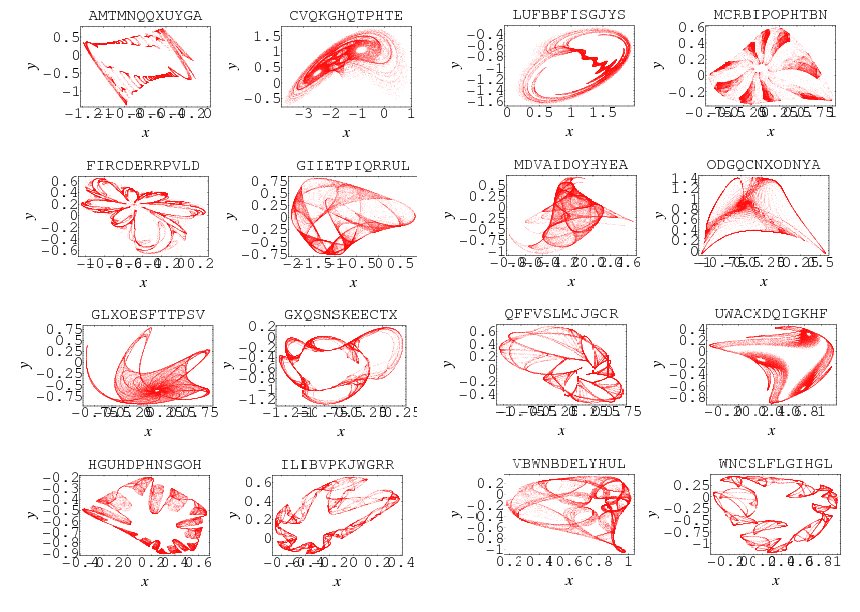
\includegraphics[scale=0.6]{figures/strange_attractors.png}
    \caption{Some strange attractors. Figures from \href{http://mathworld.wolfram.com/StrangeAttractor.html}{E. W. Weisstein}.}
\end{figure}

\subsection{Reconstructing Attractors}
In \speccite{packard1980geometry}, \citeauthor{packard1980geometry} were interested in problem of \textit{dynamical reconstruction}: from experimental observations of a turbulent fluid flow, how does one show the existence of a low-dimensional chaotic dynamical system which explains the observed behaviors? Additionally, how does one determine the dimensionality of the underlying attractor? They demonstrate their ideas using another non-linear dynamical system studied by \parencite{rossler1976equation}:

\begin{align}
    \begin{split}
        \dt{X} &= - ( Y + Z ), \\
        \dt{Y} &= X + 0.2 Y, \\
        \dt{Z} &= 0.4 + XZ - 5.7 Z.
    \end{split}
\end{align}



\begin{figure}[H]
    \centering
    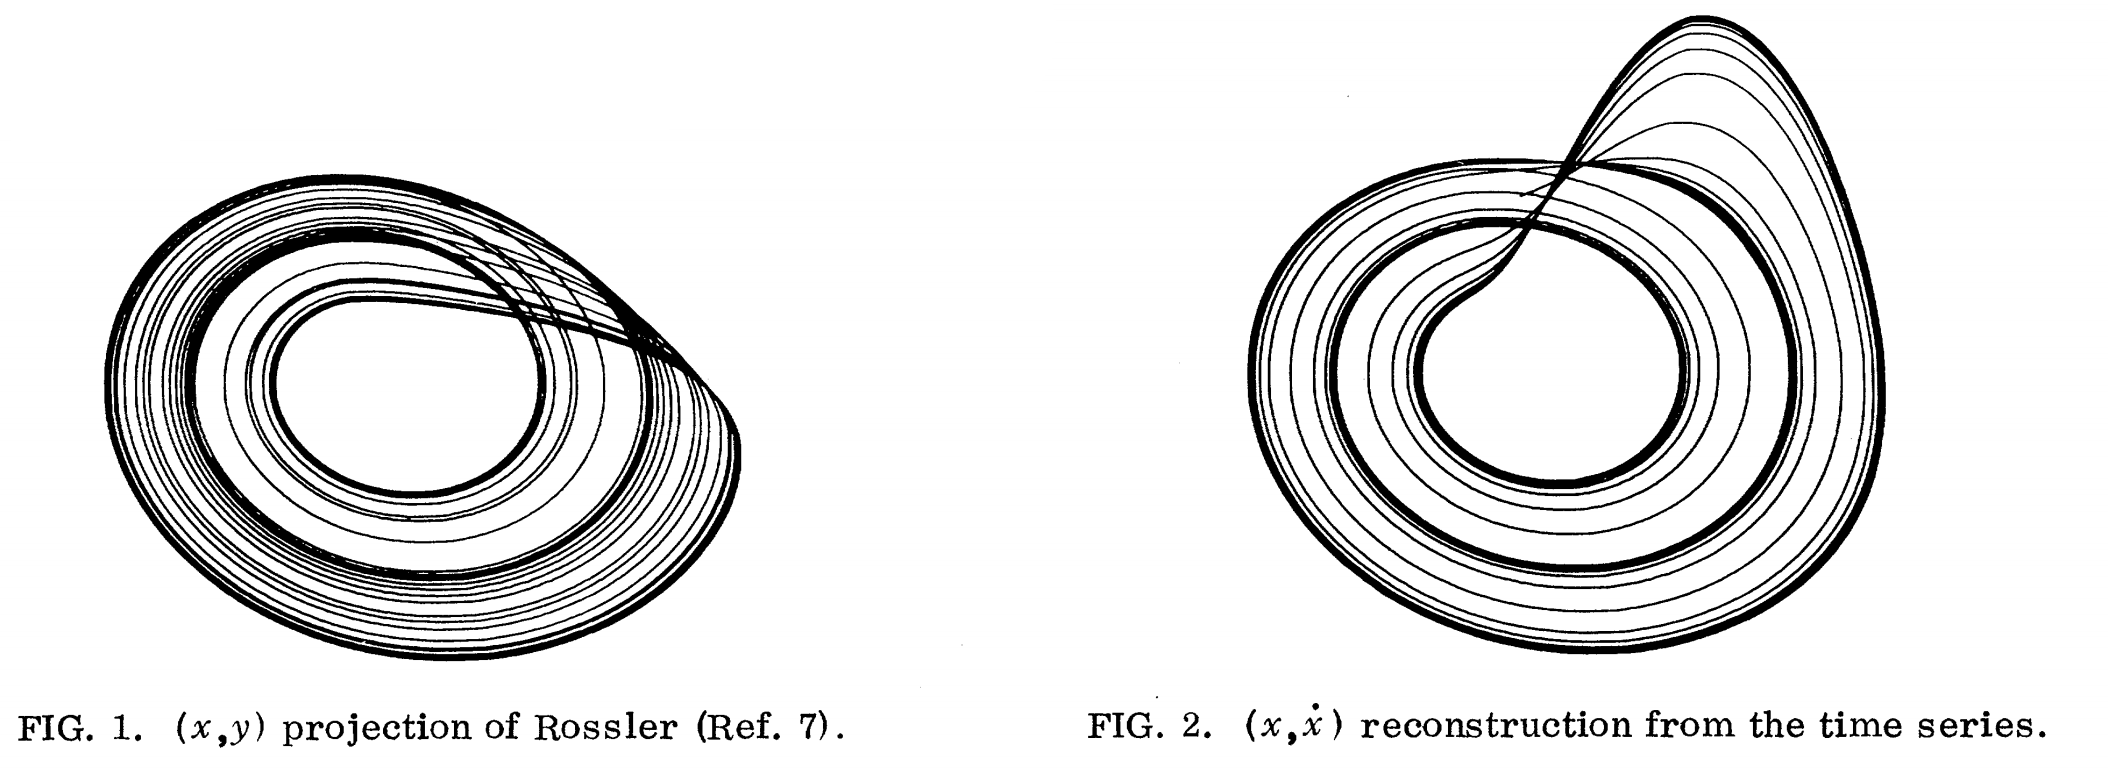
\includegraphics[scale=0.25]{figures/rossler_reconstruction.png}
    \caption{The \citeauthor{rossler1976equation} system flow projected onto the $X, Y$ plane and the induced flow of $(X, \dot X, \ddot X)$ projected onto the $X, \dot X$ plane. Figure from \parencite{packard1980geometry}.}
\end{figure}

\section{Attractors and Takens' Theorem}

\section{Selected References}

\subsection{Some Recent Developments in a Concept of Causality}

\citeauthor{granger1988some}

\subsection{Detecting Causality in Complex Ecosystems}

\citeauthor{sugihara2012detecting}

\subsection{Distinguishing Time-delayed Causal Interactions using Convergent Cross Mapping}

\citeauthor{ye2015distinguishing}

\subsection{Exact Inference of Causal Relations in Dynamical Systems}

\citeauthor{benkHo2018exact}

\clearpage
\nocite{*}
\printbibliography
\end{document}
